%% Beamer slides for:
%%   "Using LLMs in research (in September 2026)"
%%   5-minute talk. Same style as the AG DiD deck (iqss theme, Brown-red
%%   recolor, \pause overlays, momentary blue alerts, \srccite gray citations).
%% Compile with XeLaTeX. Theme files are vendored in ./theme/.

% The theme files are in ./theme/. Add the folder to the search path so the deck builds
% without TEXINPUTS (for example on Overleaf, with the compiler set to XeLaTeX).
\makeatletter
\providecommand*{\input@path}{}
\g@addto@macro\input@path{{theme/}}
\makeatother
\documentclass[11pt]{beamer}
\usepackage{amsmath,amssymb}
\usepackage{graphicx}
\usepackage{booktabs}
\usepackage{url}
\usepackage{pifont}
\usepackage{tikz}
\usepackage{environ}

\graphicspath{{figures/}}

\usepackage{appendixnumberbeamer}
\usetheme{iqss}
\setbeamertemplate{blocks}[default]   % flat blocks, no drop shadow

% ===== Brown University recolor: dark red instead of IQSS orange =====
\definecolor{brownred}{HTML}{8B1A1A}      % Brown dark red
\definecolor{iqss@orange}{HTML}{8B1A1A}   % override the theme structure/title color
\definecolor{paperwhite}{rgb}{1,1,1}
\hypersetup{allcolors=iqss@orange}

% Because this deck has its own transition frames (dark red canvas, centered
% point number and title, bullets revealed below on later clicks), we switch
% off the theme's table-of-contents section dividers.
\AtBeginSection[]{}

% ----- transition frames -----
% [plain] frame on the theme's dark red divider canvas. The number and title
% are centered on the page for title-only frames. When the frame has bullets,
% the number and title are placed in the upper part of the page at a fixed
% position on every click and the bullets fill the space below (hidden bullets
% retain their space, and nothing moves between clicks).
% #1 = point number (may be empty), #2 = title, body = optional bullets
\colorlet{citecol}{gray}
\NewEnviron{transition}[2]{%
  \setbeamercolor{background canvas}{bg=brownred}%
  \setbeamercolor{normal text}{fg=paperwhite,bg=brownred}%
  \setbeamercolor{structure}{fg=paperwhite}%
  \setbeamercolor{alerted text}{fg=paperwhite}%
  \definecolor{iqss@orange}{rgb}{1,1,1}%
  \colorlet{citecol}{paperwhite!75!brownred}%
  \frame[plain]{%
    \usebeamercolor[fg]{normal text}%
    \if\relax\detokenize\expandafter{\BODY}\relax
      \vfill
      \begin{center}
        \ifx\relax#1\relax\else
          {\usebeamerfont{title}\bfseries\fontsize{44}{48}\selectfont #1\par}\vskip 0.35em
        \fi
        {\usebeamerfont{title}\LARGE #2\par}
      \end{center}
      \vfill
    \else
      \vbox to 0.42\textheight{\vfill
        \begin{center}
          {\usebeamerfont{title}\bfseries\fontsize{44}{48}\selectfont #1\par}\vskip 0.35em
          {\usebeamerfont{title}\LARGE #2\par}
        \end{center}}%
      \vbox to 0.5\textheight{\vskip 1.2em
        \begin{center}
          \begin{minipage}{0.86\textwidth}\small\BODY\end{minipage}
        \end{center}
        \vfill}%
    \fi
  }%
}

\newcommand{\srccite}[1]{{\scriptsize\textcolor{citecol}{#1}}}
\definecolor{okgreen}{HTML}{2E7D32}
\newcommand{\good}{{\textcolor{okgreen}{\ding{51}}}\,}
\definecolor{featblue}{HTML}{1F5FA8}
\setbeamercolor{alerted text}{fg=featblue}   % one blue everywhere: alerts match \feat and figure annotations
% highlight #2 in blue only on overlay #1 (the slide where it is featured)
\newcommand{\feat}[2]{\alt<#1|handout:0>{\textcolor{featblue}{#2}}{#2}}
% roadmap numbers: same weight as the transition numbers, in Brown red on white
\newcommand{\rmapnum}[1]{\textcolor{brownred}{\textbf{#1}}}

\begin{document}

\title[Using LLMs in research]{Using LLMs in research}
\subtitle{(in September 2026)}
\author[Bilinski]{%
\small
Alyssa Bilinski, PhD \\[6pt]
\footnotesize
Department of Health Services, Policy and Practice \\
Department of Biostatistics \\
Brown University}
\date{}
\titlegraphic{}
\begin{frame}[plain]
\titlepage
\end{frame}


\begin{frame}{Six things to keep in mind}
\vfill
\pause
{\large\rmapnum{1}\quad\textbf{Use frontier models}}\par
\vfill
\pause
{\large\rmapnum{2}\quad\textbf{Experiment with these models}}\par
\vfill
\pause
{\large\rmapnum{3}\quad\textbf{Don't underestimate what AI can do}}\par
\vfill
\pause
{\large\rmapnum{4}\quad\textbf{Don't overestimate AI}}\par
\vfill
\pause
{\large\rmapnum{5}\quad\textbf{Everyone else has AI too}}\par
\vfill
\pause
{\large\rmapnum{6}\quad\textbf{Think in workflows, not tools}}\par
\vfill
\end{frame}


\section{Use frontier models}

\begin{transition}{1}{Use frontier models}
\pause
\begin{itemize}\setlength\itemsep{8pt}
\item If Claude, at least Opus, maybe Fable \pause
\item If ChatGPT, the top model, not free ChatGPT \pause
\item AI summary in a Google search is not a frontier model \pause
\item Getting much better, fast \pause
\item I worry much less about fake citations than I used to
\end{itemize}
\end{transition}


\section{Experiment with these models}

\begin{transition}{2}{Experiment with these models}
\end{transition}


\begin{frame}{Keep trying}
\pause
\begin{itemize}\setlength\itemsep{10pt}
\item What failed last month may work next month \pause
\item Try different kinds of tasks \pause
\item You get more out if you put more in \pause
\item Claude Code or Codex instead of a chat window \pause
\item Spend time on your \texttt{CLAUDE.md} or \texttt{AGENTS.md} (standing instructions for every session)
\end{itemize}
\end{frame}


\section{Don't underestimate what AI can do}

\begin{transition}{3}{Don't underestimate what AI can do}
\pause
\begin{itemize}\setlength\itemsep{8pt}
\item Getting better and better \pause
\item Recent math: Erd\H{o}s problems, a Millennium problem (disputed) \srccite{(Quanta, Aug 2026)} \srccite{(OpenAI, Sep 2026)} \pause
\item We pretend at our peril that these models can't do a lot of great things in our research
\end{itemize}
\end{transition}


\section{A couple of my favorite things}

\begin{transition}{}{A couple of my favorite things}
\end{transition}


\begin{frame}{Less time, less stress}
Many of my favorites are boring.
\medskip
\pause
\begin{itemize}\setlength\itemsep{8pt}
\item Reformat a paper for a new journal (huge time saver, just check the diff) \pause
\item Draft a response to reviewers from the comments, old version, and new version \pause
\item Play with or review code, if the code is fairly well written (takes more work) \pause
\item Copyedit, find typos, fact check, check references \pause
\item Data visualization
\end{itemize}
\end{frame}


\begin{frame}{Raise the ceiling on what you can do}
\pause
\begin{itemize}\setlength\itemsep{10pt}
\item Especially if you put more work in \pause
\item Coding \pause
\item Extracting data from the literature \pause
\item Verification costs rise \pause
\item Have several agents do the task and check it, then verify it yourself
\end{itemize}
\end{frame}


\section{Don't overestimate AI}

\begin{transition}{4}{Don't overestimate AI}
\end{transition}


\begin{frame}{Jagged frontier}
\srccite{(Dell'Acqua et al., 2023)}
\pause
\begin{itemize}\setlength\itemsep{10pt}
\item Annoying to have an RA that solves Erd\H{o}s problems in its spare time \pause
\item \ldots\ and sometimes deletes a random row of your data, or does something else unspeakably dumb \pause
\item A task that seems harder to you need not be harder for AI. The rankings differ \pause
\item Models improve. What I verify, and how, keeps changing \pause
\item But don't be stupid
\end{itemize}
\end{frame}


\section{Everyone else has AI too}

\begin{transition}{5}{Everyone else has AI too}
\end{transition}


\begin{frame}{Don't be duplicitous}
\pause
\begin{itemize}\setlength\itemsep{10pt}
\item Tools like Pangram 4 are very good at detecting AI writing \srccite{(Pangram, 2026)} \pause
\item AI writing is fine with me, if it is good writing \pause
\item I mind very bad writing that ends ``entirely human written,'' when Pangram says $100\%$ not \pause
\item AI can make pretty slides, but many unedited Claude slides are annoying. Spend time on your own formatting \pause
\item Ideally, use AI to raise the ceiling rather than the floor
\end{itemize}
\end{frame}


\section{Think in workflows, not tools}

\begin{transition}{6}{Think in workflows, not tools}
\end{transition}


\begin{frame}{Impressions change with use}
\begin{columns}[T]
\begin{column}{0.54\textwidth}
\centering
\only<1|handout:0>{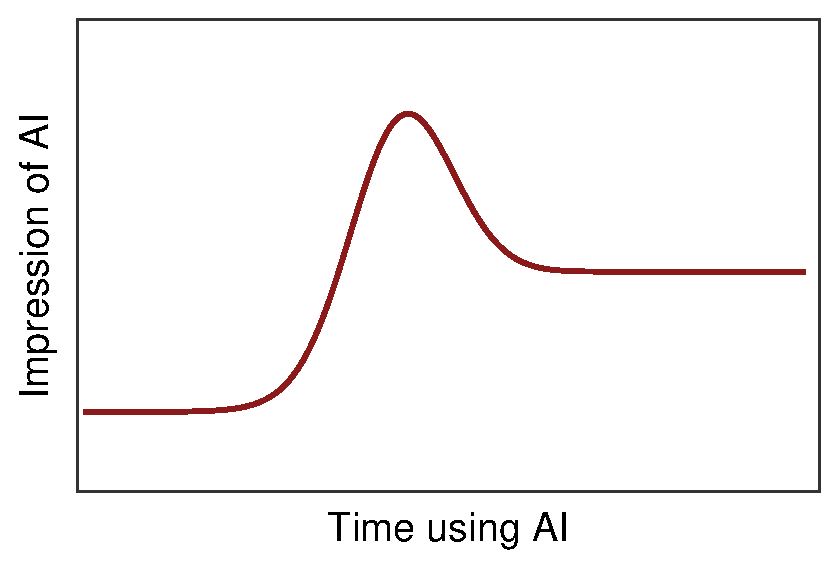
\includegraphics[width=\textwidth]{llm_curve_0.pdf}}%
\only<2|handout:0>{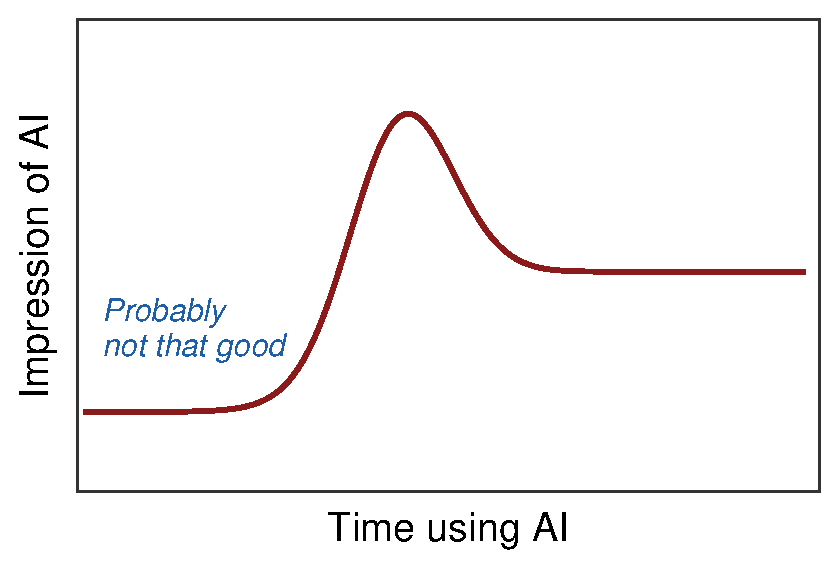
\includegraphics[width=\textwidth]{llm_curve_1.pdf}}%
\only<3|handout:0>{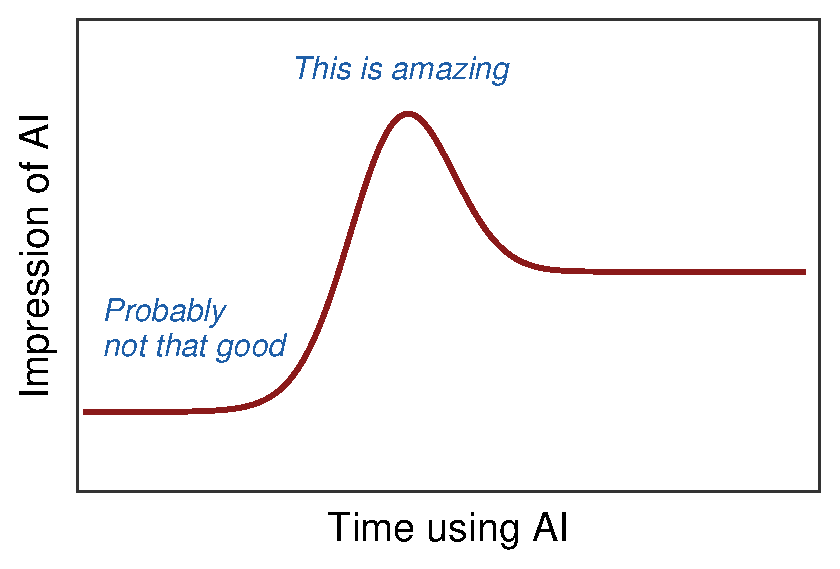
\includegraphics[width=\textwidth]{llm_curve_2.pdf}}%
\only<4-|handout:1>{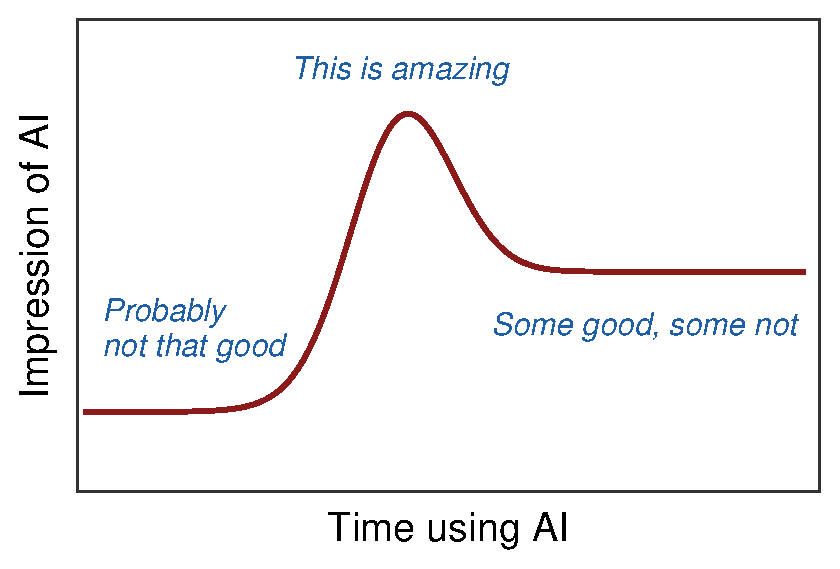
\includegraphics[width=\textwidth]{llm_curve_3.pdf}}%
\end{column}
\begin{column}{0.44\textwidth}
\pause
\begin{itemize}\setlength\itemsep{10pt}
\item Before trying: ``probably not that good'' \pause
\item First try, output optimized to look pretty: ``this is amazing'' \pause
\item Closer look: some good, some not \pause
\item Also addictive, like social media
\end{itemize}
\end{column}
\end{columns}
\end{frame}


\begin{frame}{Polarized training}
\pause
\begin{itemize}\setlength\itemsep{10pt}
\item From running: two extremes, little in between \pause
\item No AI: careful writing, often by hand, on paper, away from the computer \pause
\item Heavy AI: kick off a bunch of agents to explore data and try new things
\end{itemize}
\end{frame}


\begin{frame}{Takeaway}
\vfill
\pause
\begin{itemize}\setlength\itemsep{12pt}
\item Raise the ceiling \pause
\item Don't settle for a lazy floor
\end{itemize}
\vfill
\pause
\centering
\href{mailto:alyssa_bilinski@brown.edu}{alyssa\_bilinski@brown.edu}
\vfill
\end{frame}

\end{document}
